\documentclass[12,twoside]{mammeTFM}
%\usepackage[active]{srcltx}
\usepackage{amsthm,amsmath,amssymb,amsfonts,amscd}
\usepackage{graphicx}
\usepackage{enumerate}
\usepackage[all]{xy}
\usepackage{booktabs}
\usepackage[colorlinks=true,linkcolor=black,anchorcolor=black,citecolor=black,filecolor=black,menucolor=black,runcolor=black,urlcolor=black]{hyperref}
\usepackage{tikz}
\usepackage{xcolor}
\usepackage{float}

\usetikzlibrary{shapes}
\usetikzlibrary{positioning}
%\usepackage[usenames]{xcolor}
%\usepackage{fancyhdr}

%%%%%Author packages if necessary


% Theorem Environments: add extra ones at the end if you need it.

\newtheorem*{theoremA}{Theorem A}
\newtheorem{theorem}{Theorem}[section]

\newtheorem{proposition}[theorem]{Proposition}
\newtheorem{lemma}[theorem]{Lemma}
\newtheorem{corollary}[theorem]{Corollary}
\newtheorem{conjecture}[theorem]{Conjecture}

\theoremstyle{definition}
\newtheorem{definition}[theorem]{Definition}
\newtheorem{example}[theorem]{Example}

\theoremstyle{remark}
\newtheorem{remark}[theorem]{Remark}
\newtheorem*{remarknonumber}{Remark}
\newtheorem{observation}[theorem]{Observation}




%%%%%%%%%%%%%%%%%%
% macros/abbreviations: Include here your own.
%%%%%%%%%%%%%%%%%%

\newcommand{\N}{\ensuremath{\mathbb{N}}}


% Body of document

\titol{A Remotely-driven Hoverboard \\[3mm] With Platform Leaning Control}
\titolcurt{Leaning Control}
\authorStudent{Esteve Tarrag\'o}
\supervisors{Advisor: Enric Celaya, Tutor: Merc\`e Oll\`e}
\monthYear{September, 2019}

%\msc[2010]{Primary  	55M25, 57P10, Secondary 55P15, 57R19, 57N15.}

\paraulesclau{Dynamic, System, Control, Design}
\agraiments{
I would first like to thank my thesis advisor Prof. Enric Celaya. Enric was always 
open whenever I ran into a trouble spot or had a question about my research or 
writing. He consistently allowed this thesis to be my own work, but steered me in 
the right the direction whenever he thought I needed it.

I would also like to thank  Prof. Llu\'is Ros who was also advising me through
the first steps of the design and always gave constructive feedback.

Also this project wouldn't have been possible without my lab co-workers. I would
like to highlight three of them: I\~nigo Moreno, Sergi Hernandez and Patrick Grosch.
They teached my all kind of stuff and I am very grateful for their time.

This research opportunity was possible thanks to IRI (Institut de Robòtica i Informàtica
Industrial). They facilited my a workstation, material and a fantastic
workshop where to build my robot.
}


\abstracteng{
    This thesis is centered arround the design, construction and control of a 
    remote hoverboard. The main challenge of this project is the study of the 
    leaning control of the hoverboard platform and the restrictions it induce.

    Nowadays segways are a popular way of human transportation and there also exist segway robots. 
    Both, human-driven and autonomus segway robots have their speed determined by their inclination.
    (e.i. If you wish to go forward in a segway you should put your weight in the same direction).
    So in this systems the inclination is not a degree of freedom but a compulsary consequence from moving.
    Unblocking this degree of freedom may help two-wheel robots perform new task as mesurments, taking images 
    or samples from other inclinations, avoiding obstacles, etc.

    We have studied diferrent mechanisms to control the leaning while allowing the movement of the robot.
    Then we studied the dynamics of our system to deterimine it's dimensions and create an optimal design
    accordingly. We have also run simulations with different policies to see how our system would evolve.
    
    Finally we builded and programmed our robot so it can be remotely controlled from anywhere.
}

%%%%%%%%%
\begin{document}
\maketitle
\newpage
\tableofcontents

\section{Introduction}
In the IRI lab we have two segway robots, Tibi and Dabo show in figure
\ref{fig:Picture of Tibi and Dabo}. Both of them move the same way.
They must incline their body to compensate the wheel reaction. 
This may cause some problems when measuring distances with the sensors.
This fact also restricts the possible trajectories of the robots. 

We decided to build a prototype of segway robot that could control it's
inclination independently. The chosen robot is inspired in a \textit{segway hover-board}, 
similar to the one appearing in Figure \ref{fig:Picture of a commercial 
segway hover-board}. The two wheels are controlled with classic
control algorithms and the inclination of the central body is
controlled with a flywheel mechanism that we will discuss in section \ref{}.

\begin{figure}
	\centering
	\includegraphics[width=8cm]{img/robots-TIBI-i-DABO-IRI-red.jpg}
	\caption{Picture of Tibi and Dabo, \textit{two segway robots} }
	\label{fig:Picture of Tibi and Dabo}
\end{figure}

\begin{figure}
	\centering
	\includegraphics[width=8cm]{img/segway_hoverboard_picture.png}
	\caption{Picture of a commercial \textit{segway hover-board} }
	\label{fig:Picture of a commercial segway hover-board}
\end{figure}

\section{Initial design considerations}
The first thing we decided is the number of actuators.
Most of segway robot include two motors for the motion control but we added a third on in order to control the inclination.
We included three motors in total because we want to control three degrees of freedom (inclination and speed of both wheels).

In order to control the inclination of the platform we needed to add an external torque to the platform. We considered three methods: accelerating a flywheel, holding a pendulum in a non-vertical position and air friction with a fan. We discarded the last one due to the high speeds we needed to obtain a reasonable torque on the platform.

Both methods have strengths in different situations so we decided to build a mixed method that could combine both. 


We took two restriction in our design. The first one symmetry along the inclination axis in order to have an equilibrium in all possible inclinations without the need of external forces. We also took in consideration that the reinforcement learning algorithms starts being clumsy so none of the configurations should touch the ground. Figure \ref{fig:Side render view} illustrates this restriction.   

The design of the robot is done with the 3D design software \href{https://www.freecadweb.org/}{Free-cad}. All part files are uploaded to the GitHub repository \url{https://github.com/tarragoesteve/TFM} under the hardware folder.

You can see the main views on Figure \ref{fig:Isometric render view}, \ref{fig:Front render view}, \ref{fig:Top render view} and \ref{fig:Side render view}.

\begin{figure}
	\centering
	\includegraphics[width=10cm]{img/isometric_view.png}
	\caption{Isometric render view}
	\label{fig:Isometric render view}
\end{figure}
\begin{figure}
	\centering
	\includegraphics[width=10cm]{img/front_view.png}
	\caption{Front render view}
	\label{fig:Front render view}
\end{figure}
\begin{figure}
	\centering
	\includegraphics[width=10cm]{img/top_view.png}
	\caption{Top render view}
	\label{fig:Top render view}
\end{figure}
\begin{figure}
	\centering
	\includegraphics[width=4cm]{img/side_view.png}
	\caption{Side render view}
	\label{fig:Side render view}
\end{figure}

\subsection{Flywheel design}
\begin{figure}
	\centering
	\includegraphics[width=5cm]{img/fly_wheel_side.png}
	\caption{Fly wheel side render view}
	\label{fig:Fly wheel side render view}
\end{figure}

To control the inclination of the body two strategies are taken in to account. Creating torque by a pendulum or accelerating the flywheel. In order to experiment with both of them we designed a part to allow both configuration by placing weights in different spots, see figure \ref{fig:Fly wheel side render view}.

In order to create a configuration with maximum gravitational torque we have done the following computation. We denote the torque pendulum torque $\tau$, consider the masses are cylinders of mass $m_{cylinder}$ with radius $r_c$ and width $w$ and the radius of the flywheel is $r_f$.

Each mass weights:
\[ m_{cylinder} = \rho * w * \pi * r_c^2 \]

We neglect the mass of the flywheel structure versus the mass of the cylinders so all the gravitational torque created by the masses will be compensated with the opposite weight except for the two masses with different radius.

One of the weight can be placed along a rail. The distance to the center will vary from $r_{min} = r_c + r_{motor-axis} \approx r_c $ to $r_{max} = r_f - r_c$. 

The maximum torque takes place when these two masses are aligned horizontal with respect the ground and the movable weight is at distance $r_{min}$ from the center.

\[ \tau _{max} (r_c) =  m_{cylinder} * g * r_{max} -  m_{cylinder} * g * r_{min} =  m_{cylinder}* g * (r_f - 2 * r_c) \]

In order to maximize $\tau$ it we first compute the derivative:
\[\frac{\partial \tau _{max} (r_c)}{\partial r_c} = g *(\frac{\partial m}{\partial r_c} * (r_f - 2 * r_c) -  m_{cylinder} * 2)\]

\[ \frac{\partial  m_{cylinder}}{\partial r_c} = 2 * \rho * w * \pi *  r_c\]

An make it zero to find the maximum:

\[\frac{\partial \tau _{max} (r_c)}{\partial r_c} = 0\]

Substituting and simplifying we get:

\[\frac{\partial m}{\partial r_c} * (r_f - 2 * r_c) =   m_{cylinder} * 2 \Rightarrow 2 * \rho * w * \pi *  r_c\ * (r_f - 2 * r_c) = \rho * w * \pi * r_c^2 * 2 \]

\[ \Rightarrow r_c\ * (r_f - 2 * r_c) =  r_c^2 \Rightarrow (r_f - 2 * r_c) =  r_c \Rightarrow \boxed{r_f = 3 * r_c}\]


The circumradius $R$ from the center of a regular polygon to one of the vertices is related to the side length $s$ by:

\begin{center}
	\begin{tabular}{ c  c }
		\(\displaystyle R=\frac {s}{2* \sin{\frac {\pi} {n}}} \)
		& 
		\includegraphics[width=3cm]{img/PolygonParameters.png}
	\end{tabular}
\end{center}

In our case:
\[ R = r_f - r_c; \]
\[ s = 2 * r_c\]

Substituting in the circumradius equation we get n = 6, so we will use up 6 masses in our flywheel.
We will have a variable number of masses $N$ that we will be able to add to the flywheel as shown in the following table.
\begin{center}
	\begin{tabular}{c | c | c | c }
	 2 & 3 & 4 & 6 \\
	 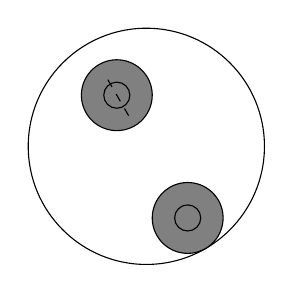
\begin{tikzpicture}[scale=0.5]
		%Circle
			\path node (center) at (0,0) {};
			\draw (center) circle (3);
		%Movable mass
			\draw[rotate=120,fill=gray] (1.5,0) circle (.9) node (moving) [draw,circle]{};
		%Guide
			\draw[dashed,rotate=120] (.9,0) -- (2.1,0);
		%Other masses
			\foreach \i in {2}
			{
				\draw[rotate=60-60*\i,fill=gray] (3-.9,0) circle (.9) node[draw,circle]{};
			}
	\end{tikzpicture}
	
	 & 
	 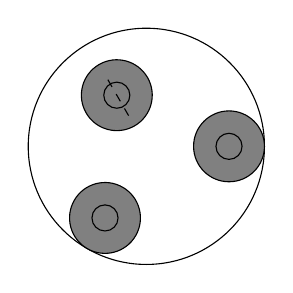
\begin{tikzpicture}[scale=0.5]
		%Circle
			\path node (center) at (0,0) {};
			\draw (center) circle (3);
		%Movable mass
			\draw[rotate=120,fill=gray] (1.5,0) circle (.9) node (moving) [draw,circle]{};
		%Guide
			\draw[dashed,rotate=120] (.9,0) -- (2.1,0);
		%Other masses
			\foreach \i in {1,3}
			{
				\draw[rotate=60-60*\i,fill=gray] (3-.9,0) circle (.9) node[draw,circle]{};
			}
	\end{tikzpicture}
	 & 
	 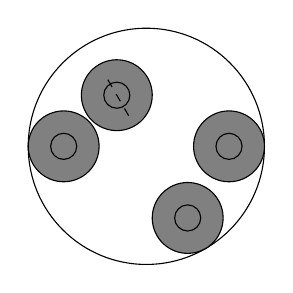
\begin{tikzpicture}[scale=0.5]
		%Circle
			\path node (center) at (0,0) {};
			\draw (center) circle (3);
		%Movable mass
			\draw[rotate=120,fill=gray] (1.5,0) circle (.9) node (moving) [draw,circle]{};
		%Guide
			\draw[dashed,rotate=120] (.9,0) -- (2.1,0);
		%Other masses
			\foreach \i in {1,2,4}
			{
				\draw[rotate=60-60*\i,fill=gray] (3-.9,0) circle (.9) node[draw,circle]{};
			}
	\end{tikzpicture} 
	&
	
	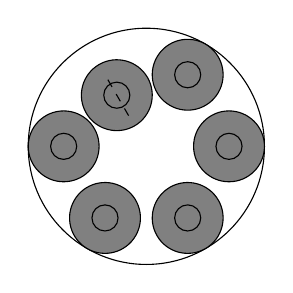
\begin{tikzpicture}[scale=0.5]
		%Circle
			\path node (center) at (0,0) {};
			\draw (center) circle (3);
		%Movable mass
			\draw[rotate=120,fill=gray] (1.5,0) circle (.9) node (moving) [draw,circle]{};
		%Guide
			\draw[dashed,rotate=120] (.9,0) -- (2.1,0);
		%Other masses
			\foreach \i in {1,2,3,4,6}
			{
				\draw[rotate=60-60*\i,fill=gray] (3-.9,0) circle (.9) node[draw,circle]{};
			}
	\end{tikzpicture}
	\\  
	\end{tabular}
	\end{center}

\section{Mechanical analysis}
\subsection{Reference frames}
In order to study the behavior of the robot we will use the following frames:
\begin{itemize}
    \item Absolute frame: From a fix object in the room. 
    \item Body frame: From the body of our robot.
\end{itemize}

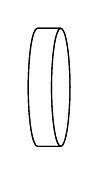
\begin{tikzpicture}[]
    \node (left_wheel) [cylinder, shape border rotate=0, draw, minimum height=1mm, minimum width=15mm] {};

    \node (right_wheel) [cylinder, shape border rotate=0, draw, minimum height=1mm, minimum width=15mm] {};

    \coordinate (left_wheel 0 0);
    \coordinate (right_wheel 10 0);



    \end{tikzpicture}


\subsection{Inclination control}
In order to keep the inclination at a certain angle we must be able to compensate all the torque being applied to the body.

Assuming that the body is well balanced and neglecting the torque generated by the friction with air, the sum of all the torques in the motor axis applied to the body is equal to the sum of the torque applied by the motors:

\[\tau_{body} = \sum \tau_{motors}\]

The torque of the motors produce a reaction in the body opposite to the torque that the motors deliver to the wheels and the flywheel.

\[\tau_{body} = -\tau_{right-wheel} -\tau_{left-wheel} -\tau_{flywheel} \]

If we want to control the inclination $\theta$, we must be able to control $\tau_{body}$ in a range $\tau_{body} \in (-\epsilon, \epsilon)$. Observe that the angular acceleration of the body is linearly dependent with the torque it receives. In the limit case $\epsilon = 0$. In order to simplify the calculations we will assume $\epsilon = 0$.

\[0 = -\tau_{right-wheel} -\tau_{left-wheel} -\tau_{flywheel} \Rightarrow \tau_{right-wheel} +\tau_{left-wheel} = -\tau_{flywheel} \]

In other words, we must compensate the torque of the wheels with the torque of the flywheel.

\subsection{Wheels torque}
The wheel torque we can induce is limited by the motor specifications. Note that the maximum torque of the motor is a function of velocity and in particular at max speed the torque is zero.

\[\tau_{motor} (w_{wheel}) \]


We assume that the wheels just roll and do no slip.
The robot is pushed by the wheels that make a force $F_{drag}$ against the ground in the contact point. See figure \ref{fig:Wheel force diagram}.

We can express the torque of the wheel as:
\[ \tau_{wheel} =min(\tau_{motor} (w_{wheel}), I_{wheel} * \dot{w}_{wheel} - F_{drag} * r_{wheel})\]
\begin{figure}[ht]
	\centering
	\includegraphics[width=10cm]{img/wheel_diagram.jpg}
	\caption{Wheel force diagram}
	\label{fig:Wheel force diagram}
\end{figure}


\subsection{Flywheel torque}

\begin{figure}
	\centering
	\includegraphics[width=10cm]{img/flywheel_diagram.jpg}
	\caption{Flywheel force diagram}
	\label{fig:Flywheel force diagram}
\end{figure}

The flywheel torque we can induce is also limited by the motor specifications. 

Assuming that a general configuration of the flywheel, see figure \ref{fig:Flywheel force diagram}. we formulate its torque the following way:


\[\tau_{flywheel} = min(\tau_{motor} (w), \ddot{\theta}*I_{flywheel}(r) + m_{cylinder} * g * (r - r_{max}) * \sin{\theta}) \]

\subsection{Motor specifications}

Here we have the factory specifications of our motors: 
\begin{itemize}
    \item Operating voltage: between 3 V and 9 V
    \item Nominal voltage: 6 V
    \item Free-run speed at 6 V: 176 RPM
    \item Free-run current at 6 V: 80 mA
    \item Stall current at 6V: 900 mA
    \item Stall torque at 6V: 5 kg·cm
    \item Gear ratio: 1:35
    \item Reductor size: 21 mm
    \item Weight: 85 g
\end{itemize}

\subsection{Hypothesis}
Assuming that the body is well balanced

\section{Optimization Setup}
In this section we will set up the requirements and the cost function we want to optimize.

\subsection{Restrictions}
The restrictions are a list of inequalities that our system has to fulfill.
The first restriction is due to the initial design requirements. Finally, the other three are 
somehow arbitrary but will help us to reduce the size of the robot.
\begin{enumerate}
\item We will place our flywheel in a hole on our robot. We don't want to touch the ground
in any configuration so:
\begin{figure}[ht]
	\centering
	\includegraphics[width=7cm]{img/flywheel_hole.jpg}
	\caption{Flywheel hole diagram}
	\label{fig:Flywheel hole diagram}
\end{figure}
\[r_{wheel}> \sqrt{(r_{flywheel} + b)^2+(\frac{h}{2})^2}\]
\item Being able  to insert the robot in to a wheel of diameter 0.5 m so:
\begin{figure}[ht]
	\centering
	\includegraphics[width=7cm]{img/external_diameter.jpg}
	\caption{External diameter diagram}
	\label{fig:External diameter diagram}
\end{figure}
\[0.25 m > \sqrt{r_{wheel}^2 + L^2/4}\]
\item We can place all electronic the devices:
\[L > 0.3m + w \]
\item Maximum weight of the robot: 5 kg
\end{enumerate}

\subsection{Requirements}
We would like our robot to reach some mechanical specifications. These are related to mechanical equations
that we will develop in the next section. They refer to the max speed, acceleration and terrain inclination the robot may achieve
while controlling its platform inclination. We have divided our specifications in two blocks
according to the two mechanisms.

\textbf{Flywheel mode}
\begin{enumerate}
	\item $\dot{y}_{max}$ (equation \ref{Maximum speed flywheel}) $> 0.1m/s$.
	\item $\ddot{y}_{max}$ (equation \ref{maximum acceleration flywheel}) $> 1m/s^2$.
	\item $sin(\alpha_{max})$ (equation \ref{Maximum angle using flywheel system}) $>0.16$.
\end{enumerate}

\textbf{Pendulum mode}
\begin{enumerate}
	\item $\dot{y}_{max}$ (equation \ref{maximum speed pendulum}) $>1m/s$.
	\item $\ddot{y}_{max}$ (equation \ref{maximum acceleration pendulum}) $>0.1m/s^2$.
	\item $sin(\alpha_{max})$ (equation \ref{Maximum angle using pendulum system}) $> 0.02$.
\end{enumerate}
	


\subsection{Cost function}
In addition to fulfilling the previous inequalities, we will adjust our design parameters [w (width of the
cylinders), N(number of cylinders), r wheel and r flywheel] to
minimize a cost function. 

We will maximize the maximum sinus in the pendulum mode 
(equation \ref{Maximum angle using pendulum system}) because
it gives the robot the capacity to deliver force in a permanent state.

And we will also maximize the square of the max speed the robot can achieve
in flywheel mode (equation \ref{Maximum speed flywheel}) because it is
proportional to the energy the robot can deliver using the flywheel at a certain moment.

Both equations try to maximize different modes so the robot we have a compromise between the two of them. 

\begin{equation}
	cost(r_{flywheel},r_{wheel},w,N) = - sin(\alpha_{max})_{pendulum} -\dot{y}^2_{max-flywheel}
	\label{eq: cost}
\end{equation}
In the next section we will find out what are the values 
of these equations with the construction parameters. 
%For reference these terms are equal to:
%\begin{equation*}
%	m_{cylinder} = \rho * w * \pi * (\frac{r_{flywheel}}{3})^2
%\end{equation*}
%\begin{equation*}
%	sin(\alpha_{max})_{pendulum} = \frac{m_{cylinder} \cdot  (r_{max} - r_{min})}{m_{total} \cdot r_{wheel}} = \frac{m_{cylinder} \cdot  (\frac{r_{flywheel}}{3})}{(m_{rest} + N \cdot m_{cylinder})\cdot r_{wheel}} 	
%\end{equation*}
%\begin{equation*}
%	\dot{y}_{max} = r_{wheel} \cdot  R \cdot  \dot{\theta}_{max} =r_{wheel} \cdot  \frac{ N \cdot  m_{cylinder} \cdot  (\frac{2\cdot r_{flywheel}}{3})^2}
%    {r_{wheel}^2\cdot (m_{rest} + N \cdot m_{cylinder}) +  2\cdot I_{wheel}} \cdot  \dot{\theta}_{max}
%\end{equation*}

\section{Flywheel break study}

This section aims to study a possible way to break the flywheel without applying torque to the platform. The idea is the following: we will leave the moving weight free.

This way, when the weight is going upward will have a larger radius than when is going downward and will produce an average moment against the movement of the flywheel.

From an energetic point of view we are transforming the rotation energy of the flywheel in to translation of the free cylinder and then realising it trough collisions.
\subsection{System of differential equations}
As described in figure \ref{fig:Flywheel force diagram} we will use two variables to describe the flywheel position: $r$, $\theta$ 

Using equation \ref{flywheel equation}:
\[\tau_{flywheel} = -\ddot{\theta}*I_{flywheel}(r) + m_{cylinder} * g * (r - r_{max}) * \sin{\theta}\]
\begin{figure}[ht]
	\centering
	\includegraphics[width=10cm]{img/cylinder_forces.png}
	\caption{Cylinder force diagram}
	\label{fig:Cylinder force diagram}
\end{figure}

As seen in figure \ref{fig:Cylinder force diagram}, we can deduce newtons equation for the distance from the cylinder to the center $r$. Note that we are adding the centrifugal force term due to the non-inertial frame.
\[\ddot{r} * m = -m * g * sin(\pi/2-\theta) + m * r * \dot{\theta}^2 \]
\[\ddot{r} = -g * sin(\pi/2-\theta) + r * \dot{\theta}^2 \]

The variables we will be using for our ODE system are: $r$,$\dot{r}$,$\theta$,$\dot{\theta}$

Note that we impose $\tau_{flywheel} = 0$ so the motor is not applying any torque.

\[
\begin{cases}
    \dot{r} = \dot{r}\\
    \ddot{r} = -g * sin(\pi/2-\theta) + r * \dot{\theta}^2\\
    \dot{\theta} = \dot{\theta}\\
    \ddot{\theta} = \frac{m_{cylinder} * g * (r - r_{max}) * \sin{\theta}}{I_{flywheel}(r)} \\    
\end{cases}
\]


Our initial conditions will be the free cylinder mass lying on the bottom of the flywheel and the flywheel turning at a speed $\theta_0$:
\[
    \begin{cases}
        r = r_{max} \\
        \dot{r} = 0\\
        \theta = \pi\\
        \dot{\theta} = \theta_0\\
    \end{cases}
\]

We will use a poincare map to simulate the bounce with the end of the guides at $r=r_{min}$ and $r=r_{max}$. At each bounce we will reduce its kinetic energy by a percentage $bounce\_percentage$ .

\subsection{Results}
The parameters of the simulation where:
\[
\begin{cases}
	r_{flywheel} = 5cm \\
	r_{wheel} = 7cm \\
	w = 2 cm \\
	\dot{\theta}_0 = 5 \pi rad/s \\
	bounce\_percentage = 0.1 \\	
\end{cases}	
\]

As we can see in figure \ref{fig:d theta t diagram} the flywheel is breaking until it becomes a pendulum and starts oscillating.

\begin{figure}[ht]
	\centering
	\includegraphics[width=10cm]{img/simulation/r_t.png}
	\caption{How the variable $r$ evolves over time}
	\label{fig:r t diagram}
\end{figure}

\begin{figure}[ht]
	\centering
	\includegraphics[width=10cm]{img/simulation/theta_t.png}
	\caption{How the variable $\theta$ evolves over time}
	\label{fig:theta t diagram}
\end{figure}

\begin{figure}[ht]
	\centering
	\includegraphics[width=10cm]{img/simulation/r_theta_t.png}
	\caption{How the variable $r$ evolves over $\theta$}
	\label{fig:r theta}
\end{figure}

\begin{figure}[ht]
	\centering
	\includegraphics[width=10cm]{img/simulation/r_theta_t_zoom.png}
	\caption{How the variable $r$ evolve over $\theta$}
	\label{fig:r theta zoom}
\end{figure}

\begin{figure}[ht]
	\centering
	\includegraphics[width=10cm]{img/simulation/d_theta_t.png}
	\caption{How the variable $\dot{\theta}$ evolve over time}
	\label{fig:d theta t diagram}
\end{figure}
\section{Dynamics}

In order to study the dynamics of the robot we will use Lagrange mechanics.

\subsection{Rectilinear movement with $r_{flywheel}$ fixed to $r_{flywheel-min}$}
To reduce the number of variables we wil study the case of rectilinear
movement by imposing that both wheels turn at the same speed. We will also set
the radius of the free weight to $r_{flywheel-min}$.

The generalized coordinates ($q$) will be:
\begin{enumerate}
	\item $\phi_{ground-wheel}$: rotation of the wheel respect the ground.
	\item $\phi_{wheel-platform}$: rotation of the platform respect the wheel.
	\item $\phi_{platform-flywheel}$: rotation of the flywheel respect the platform.
\end{enumerate}

We will use two auxiliary variables:
\begin{enumerate}
	\item $\phi_{ground-platform}=\phi_{ground-wheel}+\phi_{wheel-platform}$: rotation of the platform respect the ground.
	\item $\phi_{ground-flywheel}=\phi_{ground-platform}+\phi_{platform-flywheel}$: rotation of the flywheel respect the ground.
\end{enumerate}

The total potential energy:
\begin{equation}
	V = m_{cylinder}\cdot (r_{flywheel-min}-r_{flywheel-max}) \cdot cos(\phi_{ground-flywheel}) \cdot g	
\end{equation}


The total kinetic energy:
\begin{equation}
	T = \frac{1}{2}\cdot[\dot{\phi}_{ground-wheel}^2\cdot I_{wheel}
	+ \dot{\phi}_{ground-platform}^2 \cdot I_{platform}
	+ \dot{\phi}_{ground-flywheel}^2\cdot I_{flywheel}
	+ \dot{\phi}_{ground-wheel}^2\cdot r_{wheel}^2\cdot m_{total}]	
\end{equation}

The Lagrangian is defined as:
\begin{equation}
	L=T-V	
\end{equation}

Lagrange's equation is:
\begin{equation}
	\frac{d}{dt}(\frac{\partial L}{\partial \dot{q}_j})=
	\frac{\partial L}{\partial q_j}	+ F_{j}
\end{equation}

So in our case:
\begin{equation}
	\frac{\partial L}{\partial \dot{\phi}_{ground-wheel}}=
	\dot{\phi}_{ground-wheel} \cdot I_{wheel}
	+ \dot{\phi}_{ground-platform} \cdot I_{platform}
	+ \dot{\phi}_{ground-flywheel}\cdot I_{flywheel}
	+ \dot{\phi}_{ground-wheel}\cdot r_{wheel}^2\cdot m_{total}
\end{equation}

\begin{equation}
	\frac{\partial L}{\partial \dot{\phi}_{wheel-platform}}=
	\dot{\phi}_{ground-platform} \cdot I_{platform}
	+ \dot{\phi}_{ground-flywheel}\cdot I_{flywheel}
\end{equation}

\begin{equation}
	\frac{\partial L}{\partial \dot{\phi}_{platform-flywheel}}=
	\dot{\phi}_{ground-flywheel}\cdot I_{flywheel}
\end{equation}

We define M as the following matrix:
\begin{equation}
	\begin{pmatrix} 
		I_{wheel} + I_{platform} + I_{flywheel} + r_{wheel}^2 \cdot m_{total} &
		I_{platform} + I_{flywheel} &
		I_{flywheel}\\
		I_{platform} + I_{flywheel} &
		I_{platform} + I_{flywheel} &
		I_{flywheel}\\
		I_{flywheel} &
		I_{flywheel} &
		I_{flywheel}\\
		\end{pmatrix}
\end{equation}

In matrix form and with our generalized coordinates:
\begin{equation}
	\frac{\partial L}{\partial \dot{q}} =
	M \cdot \dot{q}
\end{equation}

\begin{equation}
	\frac{d}{dt}(\frac{\partial L}{\partial \dot{q}}) = 	M \cdot \ddot{q}	
\end{equation}

Let a be a constant:
\begin{equation}
	a = m_{cylinder}\cdot (r_{flywheel-min}-r_{flywheel-max}) \cdot g	
\end{equation}

\begin{equation}
	\frac{\partial L}{\partial q} = a \cdot sin(\phi_{ground-flywheel}) \cdot 	
	\begin{pmatrix}
	1 \\ 1 \\ 1
	\end{pmatrix}	
\end{equation}

So using Lagrange's equation we get:
\begin{equation}
	\boxed{
	M \cdot \ddot{q} = a \cdot sin(\phi_{ground-flywheel}) \cdot 	
	\begin{pmatrix}
	1 \\ 1 \\ 1
	\end{pmatrix} + F
	}
\end{equation}

\subsection{Rectilinear movement with $r_{flywheel}$ free}

The generalized coordinates ($q$) will be:
\begin{enumerate}
	\item $\phi_{ground-wheel}$: rotation of the wheel respect the ground.
	\item $\phi_{wheel-platform}$: rotation of the platform respect the wheel.
	\item $\phi_{platform-flywheel}$: rotation of the flywheel respect the platform.
	\item $r$: distance from the center of the flywheel of the free cylinder.

\end{enumerate}

We will use two auxiliary variables:
\begin{enumerate}
	\item $\phi_{ground-platform}=\phi_{ground-wheel}+\phi_{wheel-platform}$: rotation of the platform respect the ground.
	\item $\phi_{ground-flywheel}=\phi_{ground-platform}+\phi_{platform-flywheel}$: rotation of the flywheel respect the ground.
\end{enumerate}

The total potential energy:
\begin{equation}
	V = m_{cylinder}\cdot (r-r_{flywheel-max}) \cdot cos(\phi_{ground-flywheel}) \cdot g	
\end{equation}


The total kinetic energy:
\begin{multline}
	T = \frac{1}{2}\cdot[\dot{\phi}_{ground-wheel}^2\cdot I_{wheel}
	+ \dot{\phi}_{ground-platform}^2 \cdot I_{platform}
	+ \dot{\phi}_{ground-flywheel}^2\cdot I_{flywheel}(r)\\
	+ \dot{\phi}_{ground-wheel}^2\cdot r_{wheel}^2\cdot m_{total}
	+ \dot{r}^2\cdot m_{cylinder}]	
\end{multline}

The Lagrangian is defined as:
\begin{equation}
	L=T-V	
\end{equation}

Lagrange's equation is:
\begin{equation}
	\frac{d}{dt}(\frac{\partial L}{\partial \dot{q}_j})=
	\frac{\partial L}{\partial q_j}	+ F_{j}
\end{equation}

So in our case:
\begin{multline}
	\frac{\partial L}{\partial \dot{\phi}_{ground-wheel}}=
	\dot{\phi}_{ground-wheel} \cdot I_{wheel}
	+ \dot{\phi}_{ground-platform} \cdot I_{platform}\\
	+ \dot{\phi}_{ground-flywheel}\cdot I_{flywheel}(r)
	+ \dot{\phi}_{ground-wheel}\cdot r_{wheel}^2\cdot m_{total}
\end{multline}

\begin{equation}
	\frac{\partial L}{\partial \dot{\phi}_{wheel-platform}}=
	\dot{\phi}_{ground-platform} \cdot I_{platform}
	+ \dot{\phi}_{ground-flywheel}\cdot I_{flywheel}(r)
\end{equation}

\begin{equation}
	\frac{\partial L}{\partial \dot{\phi}_{platform-flywheel}}=
	\dot{\phi}_{ground-flywheel}\cdot I_{flywheel}(r)
\end{equation}

\begin{equation}
	\frac{\partial L}{\partial \dot{r}}=
	\dot{r}\cdot m_{cylinder}
\end{equation}

We define M as the following matrix:
\begin{equation}
	\begin{pmatrix} 
		I_{wheel} + I_{platform} + I_{flywheel}(r) + r_{wheel}^2 \cdot m_{total} &
		I_{platform} + I_{flywheel}(r) &
		I_{flywheel}(r)&
		0\\
		I_{platform} + I_{flywheel}(r) &
		I_{platform} + I_{flywheel}(r) &
		I_{flywheel}(r)&
		0\\
		I_{flywheel}(r) &
		I_{flywheel}(r) &
		I_{flywheel}(r) &
		0\\
		0 &
		0 &
		0 &
		m_{cylinder}\\
		\end{pmatrix}
\end{equation}

In matrix form and with our generalized coordinates:
\begin{equation}
	\frac{\partial L}{\partial \dot{q}} =
	M \cdot \dot{q}
\end{equation}

\begin{equation}
	\frac{d}{dt}(\frac{\partial L}{\partial \dot{q}}) =
	 	M \cdot \ddot{q} + \dot{M} \cdot \dot{q} 	
\end{equation}

Let's recall the definition of $I_{flywheel}(r)$
\begin{equation}
	I_{flywheel}(r)= m_{cylinder} \cdot r^2 + C	
\end{equation}


Compute the derivative
\begin{equation}
	\dot{I}_{flywheel}(r)= 2 \cdot m_{cylinder} \cdot r \cdot \dot{r} 	
\end{equation}

We compute $\dot{M}$ as the following matrix:
\begin{equation}
	\dot{M}=
	\dot{I}_{flywheel}(r) \cdot
	\begin{pmatrix} 
		1&
		1&
		1&
		0\\
		1 &
		1 &
		1&
		0\\
		1 &
		1 &
		1 &
		0\\
		0 &
		0 &
		0 &
		0\\
		\end{pmatrix}
\end{equation}

Let $a$ be::
\begin{equation}
	\frac{\partial L}{\partial q_{1..3}} = a = m_{cylinder}\cdot (r-r_{flywheel-max}) \cdot g \cdot sin(\phi_{ground-flywheel})	
\end{equation}

Let $b$ be:
\begin{equation}
	\frac{\partial L}{\partial r} = b = \cdot m_{cylinder} \cdot r  \cdot \dot{\phi}_{ground-flywheel}^2  - m_{cylinder}\cdot g \cdot cos(\phi_{ground-flywheel})	
\end{equation}

\begin{equation}
	\frac{\partial L}{\partial q} = \begin{pmatrix}
	a \\ a \\ a \\ b
	\end{pmatrix}	
\end{equation}

So using Lagrange's equation we get:
\begin{equation}
	\boxed{
	M \cdot \ddot{q} + \dot{M} \cdot \dot{q}= 
	\begin{pmatrix}
		a \\ a \\ a \\ b
		\end{pmatrix}	
 	+ F
	}
\end{equation}

\subsection{Simulations}

\section{Components}
In this section we will explain all the components
used during the building of the robot and how to get them.

\subsection{Mechanical components}
These components do not have any electronics and the important
thing about them is their mechanical function.
\subsubsection{Central Body}

Used to host the flywheel, a motor and a bearing. It also has lateral
tabs so it can easily be joined with the lateral body part.
It's 3D printed and in the same orientation you see in figure
\ref{fig: central body}.
\begin{figure}[H]
    \centering
    \includegraphics[width=10cm]{img/components/central_body.png}
    \caption{3D Model of the central body.}
    \label{fig: central body}
\end{figure}

\subsubsection{Lateral Body}
Used to host the wheel motor and the rest of the electronic components.
It also has lateral tabs so it can easily be joined with the central body part.
It's 3D printed and in the same orientation you see in figure
\ref{fig: lateral body}.
\begin{figure}[H]
    \centering
    \includegraphics[width=10cm]{img/components/lateral_body.png}
    \caption{3D Model of lateral body.}
    \label{fig: lateral body}
\end{figure}
\subsubsection{Wheels}
The wheels are 3D printed. The orientation we used to print them
is putting the motor axis vertical. Each wheel is produced by two
symmetric parts that are glued together around the motor.
\begin{figure}[H]
    \centering
    \includegraphics[width=10cm]{img/components/wheel.png}
    \caption{3D Model of a wheel.}
    \label{fig: 3D wheel}
\end{figure}
\subsubsection{Flywheel}
The flywheel is composed by 3 parts:
\begin{enumerate}
    \item 3D printed wheels very similar to the one in figure \ref{fig: 3D wheel}
    \item Steel bolts, washers and nuts.
    \item Metallic axis.
\end{enumerate}
\subsubsection{Bearings}
We are using angular balls bearing as the one seen in the figure
\ref{fig: photo bearing} to surround the flywheel axis. This bearing is
tight fit in to the 3D printed central body. The main purpose of the bearing
is to support the flywheel metal axis and help the motor with the flywheel weight
stress.
\begin{figure}[H]
    \centering
    \includegraphics[width=6cm]{img/bearing.jpg}
    \caption{Photo of a bearing.}
    \label{fig: photo bearing}
\end{figure}
\subsubsection{Reinforcements}
After we built the first prototype, we saw that the robot was suffering
from bending. So we decided to reinforce the structure with additional 3D
printed tabs and two aluminum 'U' profiles to solve the problem.

\subsection{Electronic components}
\subsubsection{Raspberry Pi}
The Raspberry Pi is a small single-board computer.
We are using Raspberry Pi 3 Model B. It has some features that we will use:
\begin{itemize}
    \item GPIO pins: General Purpose Input/Output pins are used
    \item Ethernet connection
    \item Wifi connection
    \item 5V and 3V lines
    \item DC hardware power: So we can power the Raspberry the same way as the
          other
    \item I2C: I2C is a serial protocol for two-wire interface to
          connect low-speed devices like microcontrollers. We use it to communicate
          the Raspberry Pi
\end{itemize}
\begin{figure}[H]
    \centering
    \includegraphics[width=10cm]{img/components/raspberry_pi.png}
    \caption{Raspberry Pi picture}
    \label{fig:}
\end{figure}
\begin{center}
    \begin{tabular}{ |c|c| }
        \hline
        Weight          & 42 g     \\
        \hline
        Price per unit  & 35 euros \\
        \hline
        Number of units & 1        \\
        \hline
    \end{tabular}
\end{center}
\subsubsection{Batteries}
We are using four identical batteries to power our system. They are
commercial external power supplies for smartphones. They can be recharged
via a micro-USB. We use USB cables to transmit the power to an outlet
that connects two batteries in serial that power the DC Bridges.
This bridges are powering the motors and the Raspberry.

This batteries do not work always as expected because they have
integrated security measures that disconnect them when they detect
that not power is being used.

In the other hand they incorporate many features as battery level
indicator, incorporated recharge mechanisms and on/off buttons.
\begin{center}
    \begin{tabular}{ |c|c| }
        \hline
        Weight          & 200 g    \\
        \hline
        Price per unit  & 10 euros \\
        \hline
        Number of units & 4        \\
        \hline
    \end{tabular}
\end{center}
\subsubsection{Printed Circuit Board}
In this project we tested the basic electronic with a breadboard, once we knew
the electrical components where working we decided to transfer our circuit to
a Printed Circuit Board (PCB). In particular we used a Double Sided PCB that
allows routing traces in both sides.
\begin{figure}[H]
    \centering
    \includegraphics[width=10cm]{img/components/PCB.jpg}
    \caption{Printed circuit board}
    \label{fig: PCB}
\end{figure}

\subsubsection{DC Motor}
A DC Motor is a rotary electric machine that transforms electrical energy
(in the form of direct current) into mechanical energy through electromagnetic interactions.


Here are the specifications of our three motors:

\begin{center}
    \begin{tabular}{ |c|c| }
        \hline
        Operating voltage       & between 3 V and 9 V \\
        \hline
        Free-run speed at 6 V   & 176 RPM             \\
        \hline
        Free-run current at 6 V & 80 mA               \\
        \hline
        Stall current at 6V     & 900 mA              \\
        \hline
        Stall current at 6V     & 5 kg·cm             \\
        \hline
        Gear ratio              & 1:35                \\
        \hline
        Reductor size           & 21 mm               \\
        \hline
        Weight                  & 85 g                \\
        \hline
        Price per unit          & 10 euros            \\
        \hline
        Number of units         & 3                   \\
        \hline
    \end{tabular}
\end{center}

\begin{figure}[H]
    \centering
    \includegraphics[width=6cm]{img/components/motor.jpg}
    \caption{DC Motor}
    \label{fig: DC Motor}
\end{figure}

\subsubsection{H Bridge}
An H bridge is an electronic circuit that switches the polarity of a
voltage applied to a load (in our case DC motors). This allows the motor to
go forwards and reverse.

Also it has the possibility to modulate the output power through a PWM signal.

Our particular H Bridge (L298N) is capable of supporting two motors at the same time.
This means that it has 6 input signals, 2 PWM (one for each motor) and 4 enable signals
(2 for each motor).

The input power for the H bridge is 10V but it has lost and it arrive to the motor
at around 8,5 V. Also it has a 5V power output that we use to feed the Raspberry
Pi.


\begin{figure}[H]
    \centering
    \includegraphics[width=6cm]{img/components/Hbridge.jpg}
    \caption{H Bridge}
    \label{fig: H Bridge}
\end{figure}


\subsubsection{Rotatory Encoder}
A rotary encoder, also called a shaft encoder, is an electro-mechanical device that converts the
angular position or motion of a shaft or axle to analog or digital output signals.

We programed an interruption to increment a counter to now how in what incremental position we are
and in what direction is it turning.
\subsubsection{Accelerometer}
An accelerometer is a device that measures proper acceleration. The one we are using is MPU5060.
We use the acceleration measured by the accelerometer to know in which inclination
is the platform. The accelerometer is connected to the Raspberry Pi via I2C.

\section{Control}
So far we have analyzed our system as a continuous system.
However, we are using the Raspberry Pi to control the robot, so we will
be using digital control. It's a branch of control theory that uses
digital computers to act as system controllers.

In order to sample the position and the speed we use the rotatory encoders.
They count the number of flags so there is a constant to convert them into radians.

All our digital control was made in periodical loops. To get the speed we
divided the incremental position by the period of the loop. All the controllers
are PID controllers, each of time with different inputs, constants and outputs.

A PID controller continuously calculates an error value $e(t)$ as the difference between
a desired set point and a measured process variable and applies a
correction based on proportional, integral, and derivative terms
(denoted $K_p$, $K_i$, and $K_d$ respectively).

To adjust the controller constants in all cases we used the Ziegler-Nichols method:
\footnote{Ziegler, J.G \& Nichols, N. B. (1942). "Optimum settings for automatic controllers".
 Transactions of the ASME. 64: 759-768.}

\begin{enumerate}
    \item Set all gains to zero.
    \item Increase the $K_p$ gain until the response to a disturbance is steady oscillation.
    \item Increase the $K_d$ gain until the oscillations go away (i.e. it's critically damped).
    \item Repeat steps 2 and 3 until increasing the D gain does not stop the oscillations.
    \item Set $K_p$ and $K_d$ to the last stable values.
    \item Increase the $K_i$ gain until it brings you to the set point with no oscillations desired.
\end{enumerate}

\subsection{Position control}
The input variable is the angle we would like the motor to achieve. We sense that angle
with our rotatory encoder. The output is a PWM signal and the direction the motor has to move.

The first steep was to control the position of a peg attached to the motor.
This allowed us to move the rotor from outside and also check and adjust our encoder.
In figure \ref{fig: control peg} you can see a picture of the set up we had.

\begin{figure}[H]
    \centering
    \includegraphics[width=7cm]{img/peg.png}
    \caption{Picture of the set up to control the peg.}
    \label{fig: control peg}
\end{figure}

Once knowing the constants that worked well for our peg,
we proceed the same method with the flywheel position but having a
starting point from the peg experiment.


\subsection{Speed control}
The input variable is the desired speed. We get the real speed by dividing the incremental angle
by the period (50 ms). This leaded to noisy measurements, so we decided to apply an average filter (3 samples) to
the result.

We use the motor speed control to be able to control the direction in which the robot is moving.
We transform a two-axis joystick signal (x,y) into speed set points for the PID of the wheels
 with the following formula:
\begin{equation}
    \begin{split}
    Speed_{right} = x + y \\
    Speed_{left} = x - y    
    \end{split}
\end{equation}
\subsection{Inclination control}
In order to control the inclination of the platform we also used a PID controller.
We sense the inclination of the platform with the accelerometer, and then we compute the error
as the difference between desired inclination and sensed inclination. Them, the we feed the 

\begin{itemize}
    \item In the flywheel case we simply output this error to the flywheel PWM motor signal.
    \item In the pendulum case this output is mapped to domain from -90 degrees to 90 degrees.
    Then this signal feeds another PID controller to control the position of the pendulum. We know
    the position of the pendulum by adding the inclination we sense to the rotation of the flywheel motor.
\end{itemize}

\section{Software Design}
We designed the software as modular an reusable as we could having in mind
possible future expansions of the project.
The code is divided in three main blocks: user interface (UI), planner and controller.

The UI sends the user commands to the planner, and then the planner translates that commands to
position or speed set points and sends it to the controller. Then the controller runs the control algorithms
and reports back the sensors measurements.

The reality is that the planner workload now is low but in the future it may need to compute harder problems,
as image processing, artificial intelligence or multi-robot coordination.

This three blocks are know running in three different computers but can run in different ones if needed.

You can find all the code in the GitHub repository \url{https://github.com/tarragoesteve/TFM} under the 
software folder.

\subsection{User Interface}
The user interface is a 3 column layout, the left column is for the left motor, the central column for the platform
and the right one for the right motor. As you can see in figure \ref{fig: UI}, each column has three elements,
a round progress bar to indicate the set point, a radio selection to select which parameter you wish to command and a plat
of the sensor readings.
\begin{figure}[H]
    \centering
    \includegraphics[width=12cm]{img/components/ui.png}
    \caption{Screen shoot of the UI.}
    \label{fig: UI}
\end{figure}
The user interface can be controlled by the keyboard or by a joy-stick connected to the computer. In our case
we used a PS4 remote controller connected via bluetooth to the computer.

The interface whole interface was programed with Angular, a TypeScript framework designed to code user interfaces.
It is organaized in modulus and packages that one can install, as the round progress bar. An Angular Server is 
running in the client machine that can connect to the interface via website.

\subsection{Planner}
The planner main job is to receive and sent sockets to the UI and the controller. Sockets is a method to communicate
different process across the internet with very low latency. The planner is working on a server with a public IP
so the other computers know where they have to exchange the information even if the UI or the Controller changes its IP.

\subsection{Controller}
The controller is running on the Raspberry Pi. The controller has a main file (controller.js) that reads
a configuration file (config.json) and creates instances of the components described on the configuration file.
Once all components are created, it starts different threads for each of the components.

The different components we have are: accelerometer, led, motor and stabilizer. Also we have two auxiliary classes that are
not components: PID and average filter. All the components that rely on hardware are using C++ code to optimize
the code. This code is wrapped in TypeScript classes to make an easier integration of sockets and JSON files.

\section{Conclusion}
Thinking, designing and building a prototype is a big and rewarding challenge.
There are many thinks that do not work as expected and you need to iterate again
and find a solution to the problem. Some examples are too much deformation in the platform,
too noisy speed measurements or 3D printed parts that we couldn't unpack.

On the other hand we came out with a model using the fundamental mechanics equations, but we are missing
some frictions and other forces that do not appear in our model. This made our robot behave a little bit
different from expected than the simulations. With the flywheel mode the robot can hardly start moving and with
the pendulum mode the platforms need to turn a little to start and break.

For a possible following iteration I would recommend much more powerful motors and a more robust structure.
The robot now is not behaving perfectly but can move around more or less than expected as you can see in this
\href{https://youtu.be/yWOlyIL4cP0}{video} (\href{https://youtu.be/yWOlyIL4cP0}{https://youtu.be/yWOlyIL4cP0}).

\end{document}